\documentclass{assignment}
\usepackage{relsize}
\usepackage{amsthm}
% \usepackage{amsmath}
% \usepackage{amssymb}
\usepackage{todonotes}
\usepackage{cite}
\usepackage{multirow}
\usepackage{bbding}

\author{Ritchie Cai}
\title{ELC5354 Midterm}
\date{\today}

\begin{document}

\maketitle

\begin{center}
  Choose one of the following (See \LaTeX script):
  I have redone MiniQuizes (put in numbers) 2
  % I have redone no MiniQuizes
\end{center}

\begin{itemize}
\item The exam is due on midnight one week from the date above.
\item Your solution is to be written in \LaTeX. The \LaTeX file and the corresponding pdf file is to be emailed to \verb"Robert_Marks@Baylor.edu" by the deadline. It's a good idea to ask for a receipt for your email.
\item Show your work.
\item No human resource will be consulted in the execution of the exam.
\end{itemize}


\section*{Exam}

\textbf{1.} Let's assume a man wearing a boy scout leader's uniform has a son.
In a conversation, you learn that he has two children.

\begin{enumerate}[(a)]
\item What is the probability that the man has two sons? \footnote{Assume the chances of having a boy or a girl at 50-50.} (Hint: It is not $\frac{1}{2}$).\\
  \textbf{Solution:}\\
  The probability table is given as follows:

  \begin{tabular}{| c | c | c | c |}
    \hline
    First                 & Second  &              & \multirow{2}{*}{Probability}\\
    born                  & born    &              & \\
    \hline
    \multirow{2}{*}{boy}  & boy     & \Checkmark   & $1/3$ \\
    \cline{2-4}
                          & girl    &  \Checkmark  & $1/3$\\
    \hline
    \multirow{2}{*}{girl} & boy     &  \Checkmark  & $1/3$\\
    \cline{2-4}
                          & girl    & \XSolidBrush & \\
    \hline
  \end{tabular}

  From the table we can see that the probability of two boys given that we know he has one boy is $1/3$.
  \hfill $\blacksquare$ \\
\item In addition to this information, the man says his son was born between noon and midnight.
  \footnote{We assume the chances of being born between noon and midnight 50-50.}
  Show that this additional information\footnote{If the man has two sons, we interpret this to mean that at
    least one of his sons was born between noon and midnight. Maybe both.}
  increases the probability that both of the man's sons are male.\\
  \textbf{Solution:}\\
  The probability table is given as follows, morning represent after mid night before noon, and evening represent
  otherwise, so he meant his son is borning in the \underline{evening} in this morning / evening term.

  \begin{tabular}{| c | c | c | c | c | c |}
    \hline
    first                 & time                     & second                & time    &    & \multirow{2}{*}{Probability}\\
    born                  &                          & born                  &         &    & \\
    \hline
    \multirow{8}{*}{boy}  & \multirow{4}{*}{morning} & \multirow{2}{*}{boy}  & morning & \XSolidBrush & \\
    \cline{4-6}
                          &                          &                       & evening & \Checkmark & $1/7$\\
    \cline{3-6}
                          &                          & \multirow{2}{*}{girl} & morning & \XSolidBrush & \\
    \cline{4-6}
                          &                          &                       & evening & \XSolidBrush & \\
    \cline{2-6}
                          & \multirow{4}{*}{evening} & \multirow{2}{*}{boy}  & morning & \Checkmark & $1/7$\\
    \cline{4-6}
                          &                          &                       & evening & \Checkmark & $1/7$\\
    \cline{3-6}
                          &                          & \multirow{2}{*}{girl} & morning & \Checkmark & $1/7$\\
    \cline{4-6}
                          &                          &                       & evening & \Checkmark & $1/7$\\
    \hline
    \multirow{8}{*}{girl} & \multirow{4}{*}{morning} & \multirow{2}{*}{boy}  & morning & \XSolidBrush & \\
    \cline{4-6}
                          &                          &                       & evening & \Checkmark & $1/7$\\
    \cline{3-6}
                          &                          & \multirow{2}{*}{girl} & morning & \XSolidBrush & \\
    \cline{4-6}
                          &                          &                       & evening & \XSolidBrush & \\
    \cline{2-6}
                          & \multirow{4}{*}{evening} & \multirow{2}{*}{boy}  & morning & \XSolidBrush & \\
    \cline{4-6}
                          &                          &                       & evening & \Checkmark & $1/7$\\
    \cline{3-6}
                          &                          & \multirow{2}{*}{girl} & morning & \XSolidBrush & \\
    \cline{4-6}
                          &                          &                       & evening & \XSolidBrush & \\
    \hline
  \end{tabular}

  From the table above we can see that out of 7 possible outcomes, three of them are 2 boys
  and at least one of them is born in the evening, so the probability is $3/7$. \hfill $\blacksquare$
\end{enumerate}
\vspace{0.5in}


\textbf{2.} Consider the stochastic process
  $$X(t)= \cos (2 \pi t + \Theta  )$$
  where $\Theta$ is  a random variable uniform on $(-\pi, \pi)$.
  \begin{enumerate}
  \item Is $X(t)$ WSS?
    \begin{enumerate}
    \item If not, why?
    \item If so, what is the average power of $X(t)$ on the interval $0\leq u \leq 1.5$? On $1.5\leq u \leq 27$?
    \end{enumerate}
  \item Is $X(t)$ stationary in the strict sense?
  \item If $X(t)$ mean ergodic?
  \end{enumerate}
  Explain each answer. \\

  \textbf{Solution:}\\

  \begin{align*}
    \mu = E[X(t)] & = E[\cos (2 \pi t + \Theta  )] \\
                  & = \int_{-\pi}^{\pi} \cos (2 \pi t + \theta  ) \df{1}{2 \pi} d\theta \\
                  & = \df{1}{2 \pi} \int_{-\pi}^{\pi} \cos (2 \pi t + \theta  ) d\theta  = 0 \\
    \text{autocorrelation} & = E[\textbf{x($t$)x($\tau$)}]
                             = E[\cos (2 \pi t + \theta  )\cos (2 \pi \tau + \theta  )] \\
                  & = \frac{1}{2}E[\cos (2 \pi (t - \tau)) + \cos (2\pi t + 2\pi \tau + 2\theta)]\\
    \shortintertext{Since:}
    E[\cos (2\pi t + 2\pi \tau + 2\theta)]
                  & = \df{1}{2\pi} \int_{-\pi}^{\pi} \cos (2\pi t + 2\pi \tau + 2\theta) d\theta = 0 \\
    \shortintertext{We have:}
    E[\textbf{x($t$)x($\tau$)}] & = \df{1}{2}\cos(2\pi (t - \tau)) = R(t - \tau)
  \end{align*}

  \textbf{Answer for (1):}
  Since $E[X(t)]$ is constant, and $E[X^2(t)] = 0$. $X(t)$ is WSS.
  \begin{align*}
    \ol{P} = E[X^2(t)] = R_X(0)
    & = \frac{1}{2}E[\cos (2 \pi (t - t)) + \cos (4\pi t + 2\theta)]\\
    & = \frac{1}{2}E[1 + \cos (2\theta)] \\
    \shortintertext{On interval $0\leq u \leq 1.5$:}
    \frac{1}{2}E[1 + \cos (2\theta)]
    & = \df{1}{2} + \df{1}{4\pi}\int_0^{1.5}\cos (2\theta) d\theta \\
    & = \df{1}{2} + \df{1}{4\pi}\left[ \df{\sin(2\theta)}{2} \right]_0^{1.5}
      = \df{1}{2} + \df{1}{4\pi}\left[ \df{\sin(3)}{2} \right]
      \approx 0.505615 \\
    \shortintertext{On interval $1.5\leq u \leq 27$:}
    & = \df{1}{2} + \df{1}{4\pi}\int_{1.5}^{27}\cos (2\theta) d\theta \\
    & = \df{1}{2} + \df{1}{4\pi}\left[ \df{\sin(2\theta)}{2} \right]_{1.5}^{27}
      = \df{1}{2} + \df{1}{4\pi}\left[ \df{\sin(54)- sin(3)}{2} \right]
      \approx 0.472152
  \end{align*}

  \textbf{Answer for (2)}\\
  Since $\Theta$ is uniform, thus it's time invariant. So $X(t)$ should be SSS as well. \\


  \textbf{Answer for (3)}\\
  In this case, $$\frac{1}{T} \int_0^T X(t) dt$$ doesnt not necessarily
  goes to 0 as $T \rightarrow \infty$, so it's not mean ergodic.\\
\textbf{3. MATLAB fun.} Digitally generate a large number of random probability density functions. An example might be\\
\begin{center}
  \texttt{    S=rand(N,1);}  \\
  \texttt{    fX=S/sum(S);} \\
\end{center}
The value or $N$ can vary for each density.
\begin{enumerate}[(a)]
\item  Evaluate the mean and variance of each density.\\
  \textbf{Solution:}\\
  Code segment used is shown in listing~\ref{lst:p3a}, result is shown in figure~\ref{fig:p3a}
  \CodeSnippet{matlab}{Code used to generate all the pics}{lst:p3a}{../src/matlab/problem3.m}{1}{48}
  \begin{figure}[!h]
    \begin{center}
      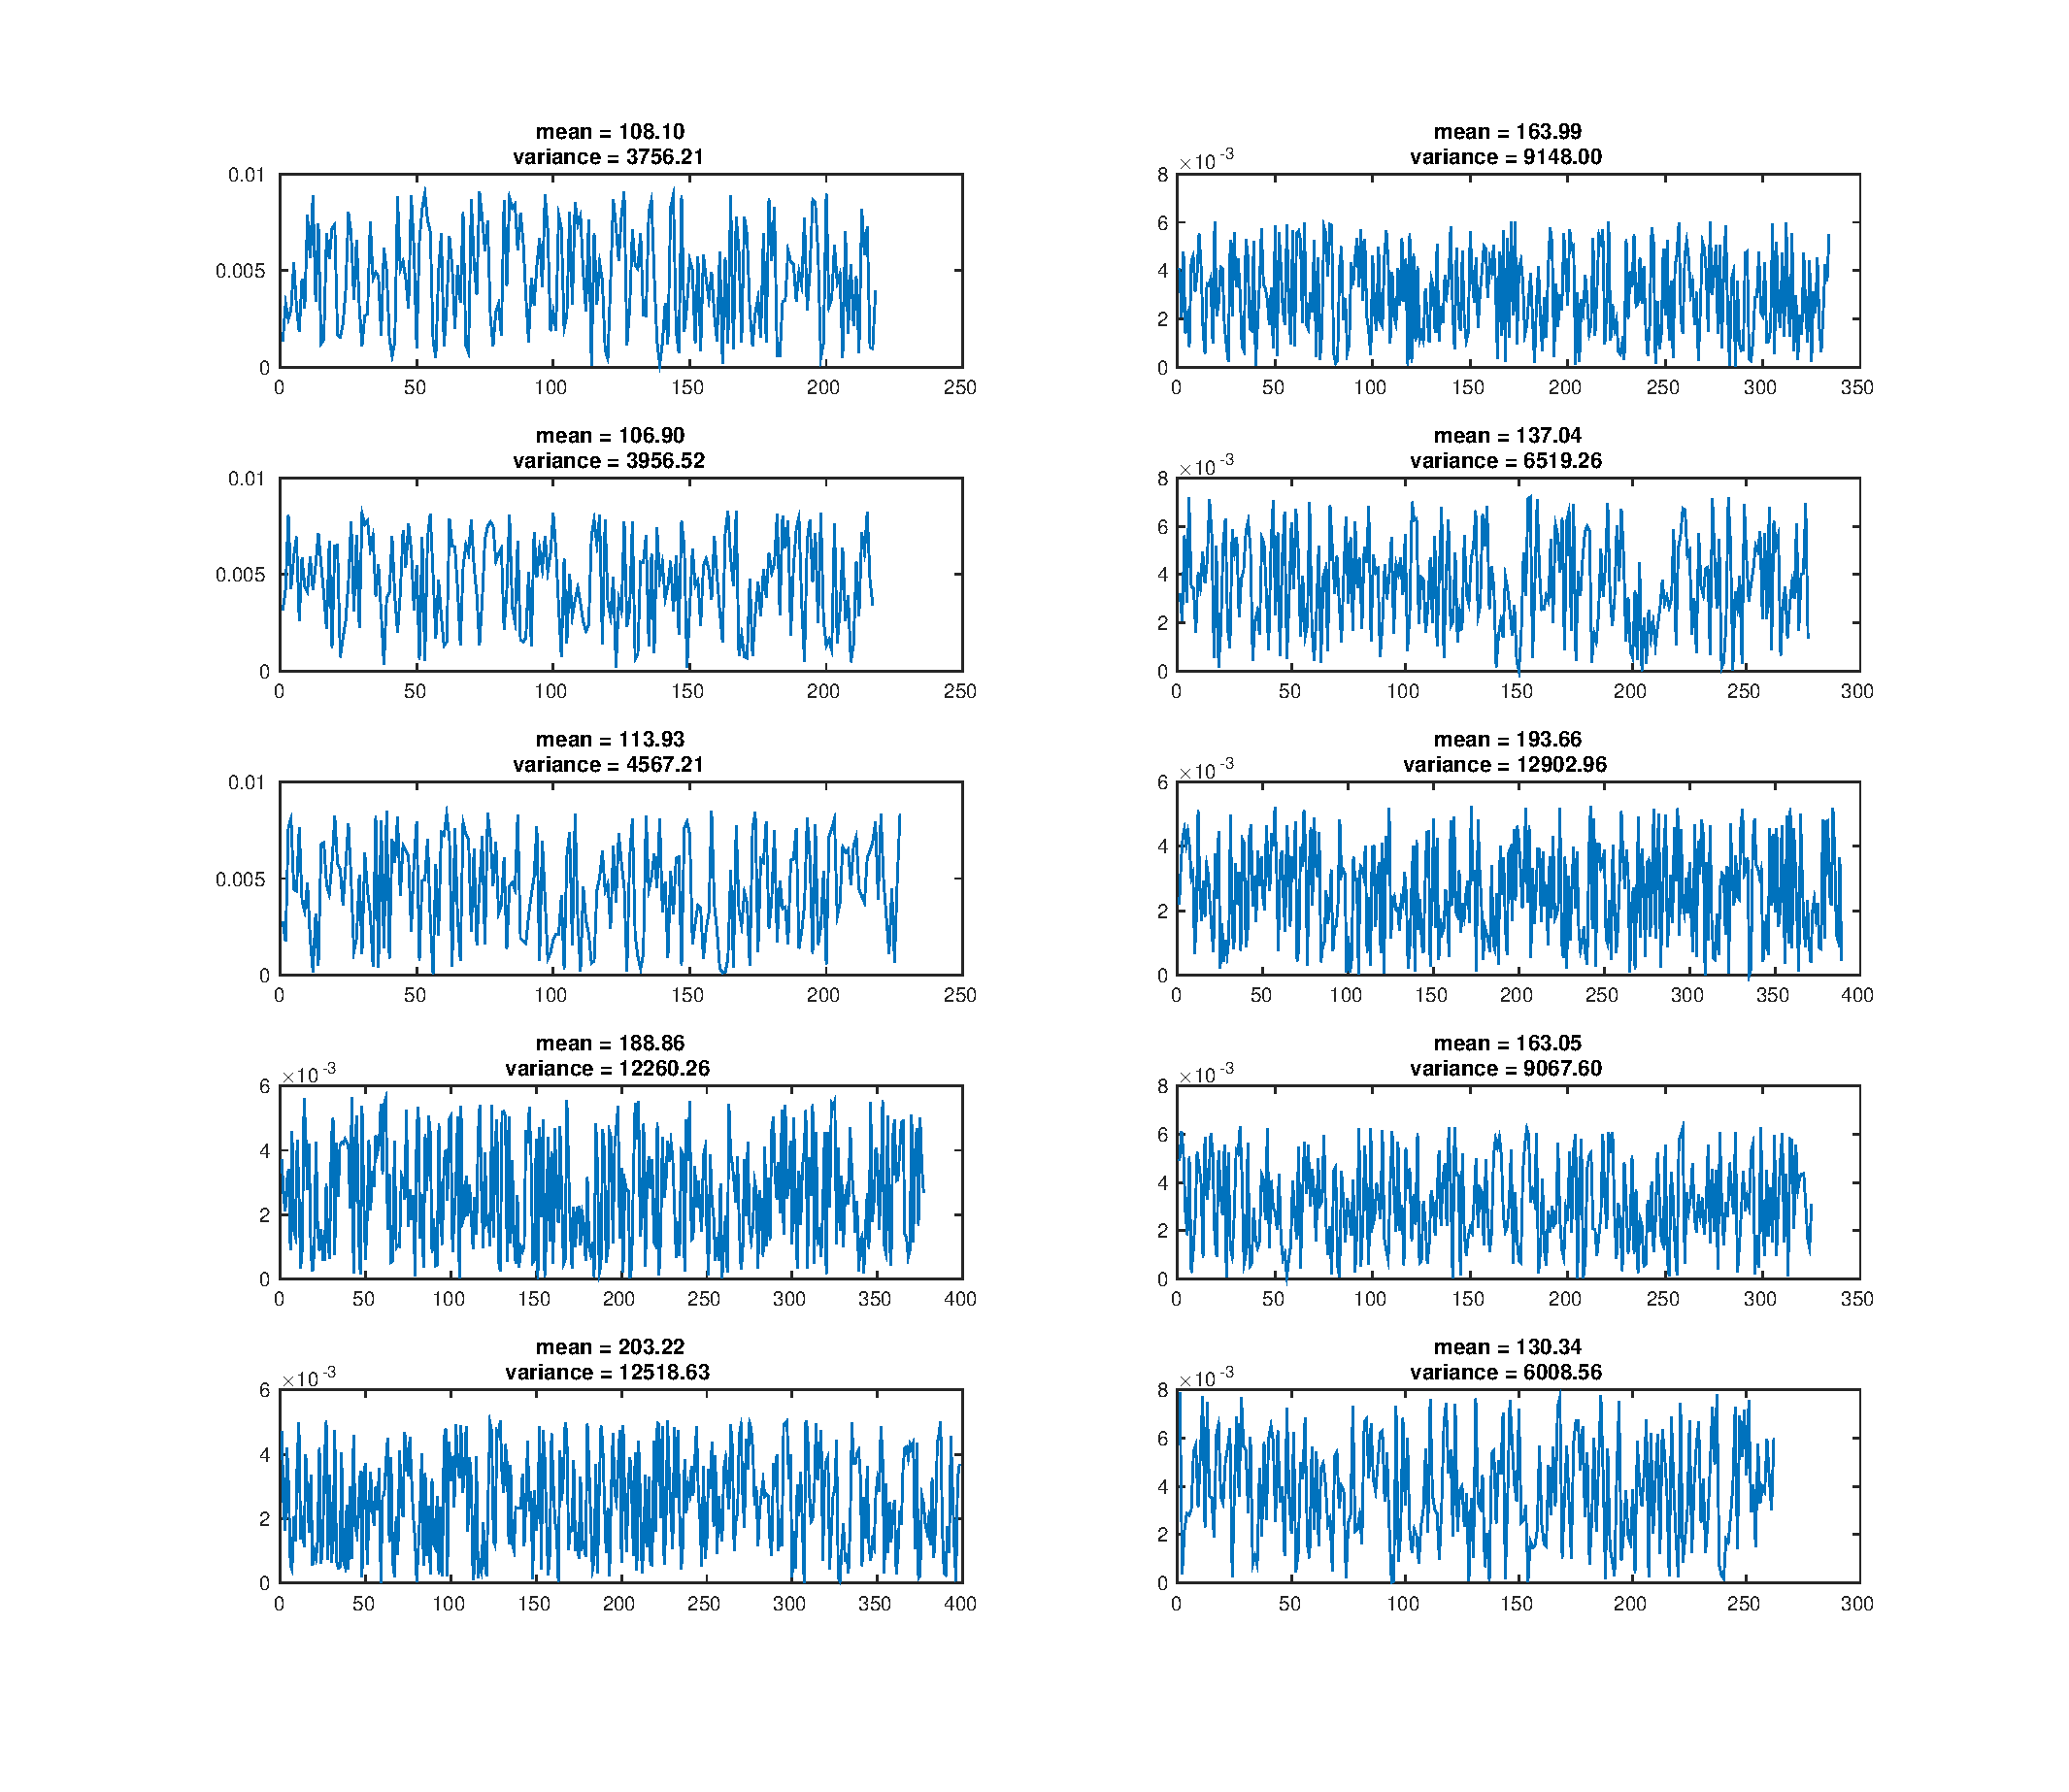
\includegraphics[width=6in]{random_distributions.eps}
    \end{center}
    \caption{Generated random distributions with their means and variances calculated.}
    \label{fig:p3a}
  \end{figure}

\item  Convolve the densities. There is a MATLAB function called \\
  \begin{center}
    \texttt{    conv;}    \\
  \end{center}
  Code segment contuned from part (a) is shown in listing~\ref{lst:p3b}
  \CodeSnippet{matlab}{Convolve all the distributions}{lst:p3b}{../src/matlab/problem3.m}{49}{70}

\item  Calculate the mean and variance of the convolution and verify the mean is the sum of the means and the variance is the sum of the variances.
  \CodeSnippet{matlab}{Code used to generate all the pics}{lst:problem3}{../src/matlab/problem3.m}{71}{79}

  outputs:
  \color{lightgray}
\begin{verbatim}
difference of mean     : 9.00
difference of variance : 0.00
\end{verbatim}
  \color{black}

\item  On the same graph, plot the convolution and the Gaussian approximation using the
  central limit theorem.
  \CodeSnippet{Matlab}{Code used to generate all the pics}{lst:problem3}{../src/matlab/problem3.m}{80}{86}
  \begin{figure}[!h]
    \begin{center}
      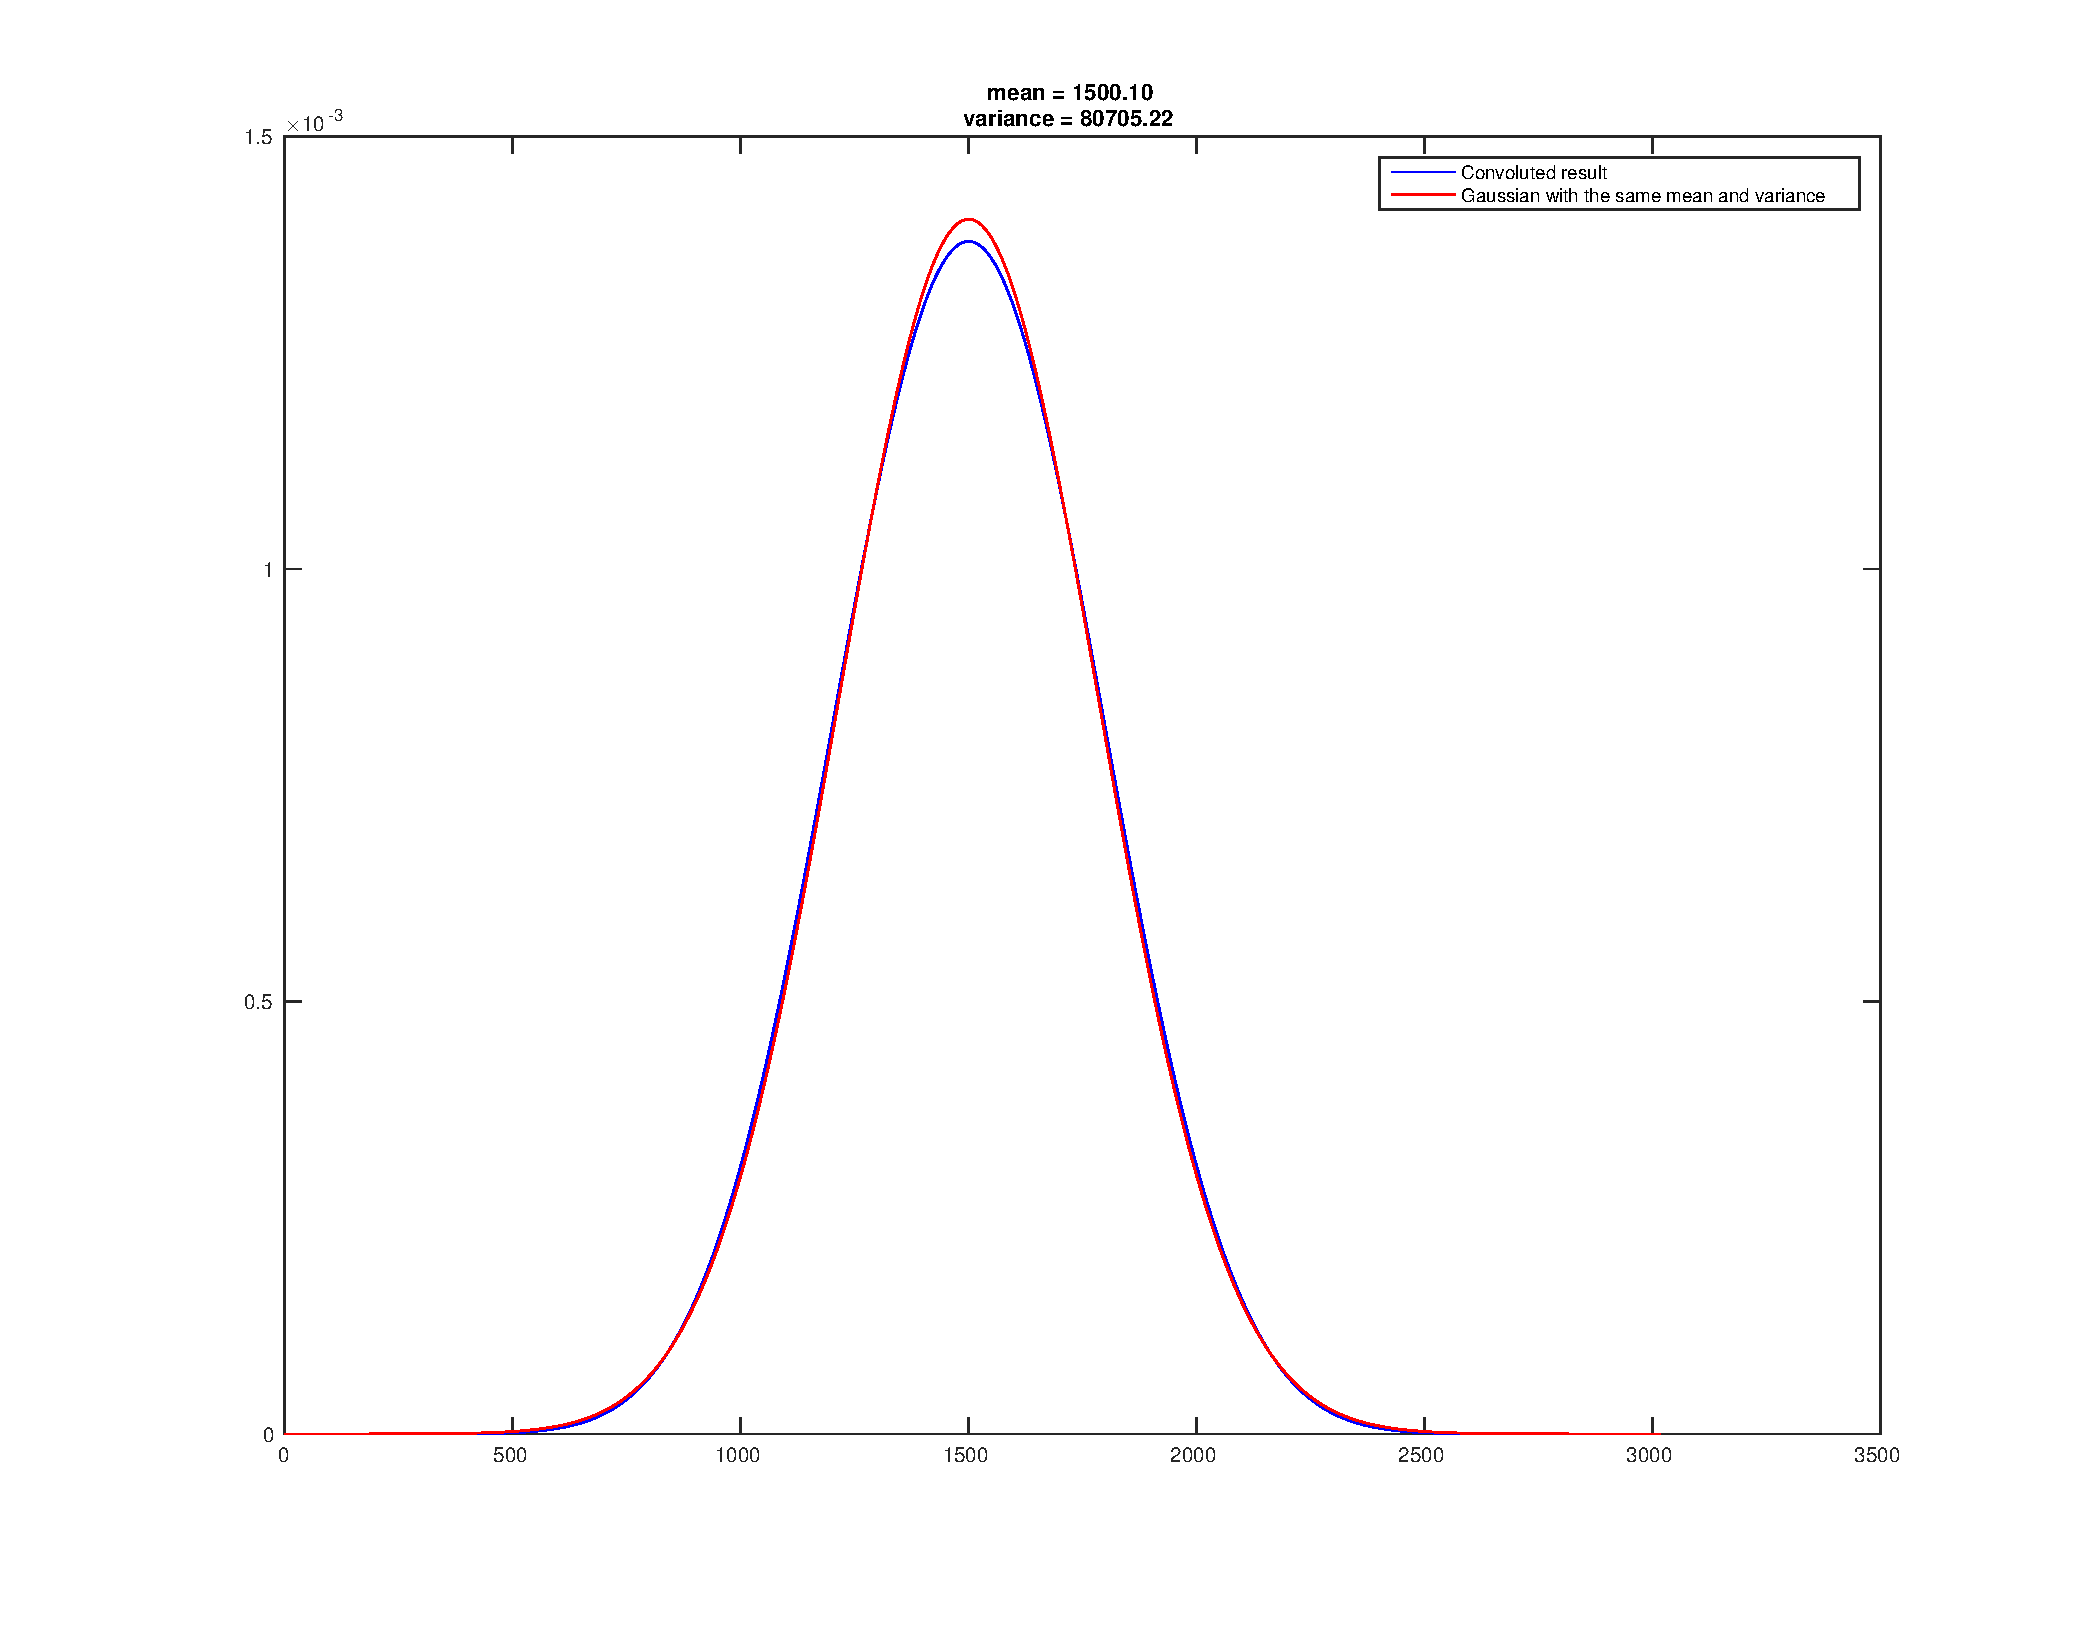
\includegraphics[width=6in]{gaussian.eps}
    \end{center}
      \caption{Convoluted distribution and gaussian pdf withe the same mean and variance}
      \label{fig:conv_gauss}
  \end{figure}
\end{enumerate}




\textbf{4.} Let $X(t)$ be the Poisson counting process with parameter $\lambda$.
  \begin{enumerate}
  \item Let
    $$ Y(t) = X(t) - \lambda t .$$
    Evaluate the mean and autocorrelation of $Y(t)$.\\
    \textbf{Answer:}\\
    \begin{align*}
      X(t) & = \df{e^{-\lambda t}(\lambda t)^k}{k!}\\
      \shortintertext{Mean:}
      E[Y(t)] & = E[X(t) - \lambda t] = E[X(t)] - E[\lambda t] = \lambda t - \lambda t = 0 \\
    \end{align*}
    Let $\tau > t$, since random variable $\textbf{x}(t)$ and $\textbf{x}(\tau) - \textbf{x}(t)$ are independent, we have
    \begin{align*}
      E[\textbf{x}(t)(\textbf{x}(\tau) - \textbf{x}(t))] & = E[\textbf{x}(t)]E[\textbf{x}(\tau) - \textbf{x}(t)] \\
                                                         & = \lambda t (\lambda \tau - \lambda t) \\
                                                         & = \lambda^2t\tau - \lambda^2t^2
    \end{align*}
    Thus
    \begin{align*}
      E[X(t)X(\tau)] & = E[X(t)(X(t) + X(\tau) - X(t))] \\
                     & = E[X^2(t) + X(t)(X(\tau) - X(t))] \\
                     & = \lambda^2t^2  + \lambda t + \lambda^2t\tau - \lambda^2t^2\\
                     & = \lambda t + \lambda^2t\tau \\
      R(t, \tau) & = E[Y(t)Y(\tau)] = E[(X(t) - \lambda t)(X(\tau) - \lambda \tau)] \\
                     & = E[X(t)X(\tau)] - \lambda \tau E[X(t)] - \lambda t E[X(\tau)] + \lambda^2 t \tau \\
                     & = \lambda t + \lambda^2 t \tau - \lambda^2 \tau t - \lambda^2 t \tau + \lambda^2 t \tau \\
                     & = \lambda t
    \end{align*}
    $\hfill\blacksquare$
  \item Let
    $$Z(t) = \frac{dY(t)}{dt}.$$
    Evaluate the mean and autocorrelation of $Z(t)$.\\
    \textbf{Answer:}\\
    \begin{align*}
      e^{\lambda} & = \sum_{k=1}^{\infty} k(k-1)(k-2) \df{\lambda^{k-3}}{k!}
                    = \sum_{k=1}^{\infty} (k^3 - 3k^2 + 2k) \df{\lambda^{k-3}}{k!} \\
                  & = \df{1}{\lambda^3} \left[ \sum_{k=1}^{\infty} k^3 \df{\lambda^k}{k!}
                    - 3 \sum_{k=1}^{\infty} k^2 \df{\lambda^k}{k!}
                    + 2 \sum_{k=1}^{\infty} k \df{\lambda^k}{k!} \right] \\
                  & = \df{1}{\lambda^3} \left[ \sum_{k=1}^{\infty} k^3 \df{\lambda^k}{k!}
                    -3e^{\lambda} (\lambda^2 + \lambda) + 2e^{\lambda}\lambda \right] \\
      \sum_{k=1}^{\infty} k^3 \df{\lambda^k}{k!}
                  & = \lambda^3e^{\lambda} + 3e^{\lambda}\lambda^2 + e^{\lambda}\lambda
                    = e^{\lambda}(\lambda^3 + 3\lambda^2 + \lambda)
    \end{align*}
    \begin{align*}
      Z(t) & = \df{dY(t)}{dt} = \df{dX(t)}{dt} - \lambda
             = \df{d}{dt} \left(\df{e^{-\lambda t} (\lambda t)^k}{k!}\right) - \lambda \\
           & = -\lambda \df{e^{-\lambda t} (\lambda t)^k}{k!} +
             \lambda \df{e^{-\lambda t} (\lambda t)^{k-1}}{(k-1)!} - \lambda \\
      \shortintertext{Let:}
      F(t) & = \df{dX(t)}{dt}
             = -\lambda \df{e^{-\lambda t} (\lambda t)^k}{k!} + \lambda \df{e^{-\lambda t} (\lambda t)^{k-1}}{(k-1)!} \\
      \shortintertext{Mean:}
      E[F(t)] & = \sum_{k=1}^{\infty} k \left( \lambda \df{e^{-\lambda t} (\lambda t)^{k-1}}{(k-1)!}
                -\lambda \df{e^{-\lambda t} (\lambda t)^k}{k!} \right) \\
           & = e^{-\lambda t} \left( \sum_{k=1}^{\infty} k \df{\lambda (\lambda t)^{k-1}}{(k-1)!}
             - \lambda \sum_{k=1}^{\infty} k \df{(\lambda t)^k}{k!}\right) \\
           & = e^{-\lambda t} \left( \df{1}{t}\sum_{k=1}^{\infty} k^2 \df{(\lambda t)^{k}}{k!}
             - \lambda \sum_{k=1}^{\infty} k \df{(\lambda t)^k}{k!}\right) \\
           & = e^{-\lambda t} \left(  \df{1}{t} e^{\lambda t}(\lambda^2 t^2 + \lambda t) - e^{\lambda t}\lambda^2 t\right) \\
           & = \lambda^2 t - \lambda^2 + \lambda \\
      \shortintertext{also}
      E[F^2(t)] & = \sum_{k=1}^{\infty} k^2 \left( \lambda \df{e^{-\lambda t} (\lambda t)^{k-1}}{(k-1)!}
                -\lambda \df{e^{-\lambda t} (\lambda t)^k}{k!} \right) \\
           & = e^{-\lambda t} \left( \sum_{k=1}^{\infty} k^2 \df{\lambda (\lambda t)^{k-1}}{(k-1)!}
             - \lambda \sum_{k=1}^{\infty} k^2\df{(\lambda t)^k}{k!}\right) \\
           & = e^{-\lambda t} \left( \df{1}{t}\sum_{k=1}^{\infty} k^3 \df{(\lambda t)^{k}}{k!}
             - \lambda \sum_{k=1}^{\infty} k^2 \df{(\lambda t)^k}{k!}\right) \\
           & = e^{-\lambda t} \left(  \df{1}{t} e^{\lambda t}(\lambda^3t^3 + 3\lambda^2t^2 + \lambda t)
             - e^{\lambda t}\lambda (\lambda^2 t^2 + \lambda t)\right) \\
           & = \lambda^3t^2 + 3 \lambda^2t + \lambda - \lambda^3t - \lambda^2 \\
           & = \lambda^3t^2 - \lambda^3t + 3 \lambda^2t - \lambda^2 + \lambda \\
      \shortintertext{So, we have}
      E[Z(t)] & = E\left[ F(t) - \lambda \right] = E[F(t)] - \lambda = \lambda^2 t - \lambda^2\\
      \shortintertext{Let $\tau > t$}
      E[F(t)F(\tau)] & = E[F(t)(F(t) + F(\tau) - F(t))] \\
           & = E[F^2(t)] + E[F(t)]E[F(\tau) - F(t)] \\
           & = \lambda^3t^2 - \lambda^3t + 3 \lambda^2t - \lambda^2 + \lambda
             + (\lambda^2 t - \lambda^2 + \lambda)
             (\lambda^2 t - \lambda^2 + \lambda - \lambda^2 t + \lambda^2 - \lambda) \\
           & = \lambda^3t^2 - \lambda^3 t + 3 \lambda^2t - \lambda^2 + \lambda
             + (\lambda^2 t - \lambda^2 + \lambda)(\lambda^2 \tau - \lambda^2 t) \\
           & = \lambda^3 t^2 - 2 \lambda^3 t + 3 \lambda^2 t - \lambda^2 + \lambda +
             \lambda^4 t \tau - \lambda^4 t^2 - \lambda^4 \tau + \lambda^4 t + \lambda^3 \tau\\
           & = \lambda^4 t \tau - \lambda^4 t^2 - \lambda^4 \tau + \lambda^4 t
             + \lambda^3 t^2 - 2 \lambda^3 t + \lambda^3 \tau + 3 \lambda^2 t - \lambda^2 + \lambda \\
      \shortintertext{}
      R(t, \tau) & = E[Z(t)Z(\tau)] = E[(F(t) - \lambda)(F(\tau) - \lambda)] \\
           & = E[F(t)F(\tau) - \lambda F(t) - \lambda F(\tau) + \lambda^2] \\
           & = \lambda^4 t \tau - \lambda^4 t^2 - \lambda^4 \tau + \lambda^4 t
             + \lambda^3 t^2 - 2 \lambda^3 t + \lambda^3 \tau + 3 \lambda^2 t - \lambda^2 + \lambda \\
           & \quad - \lambda (\lambda^2 t - \lambda^2 + \lambda) - \lambda (\lambda^2 \tau - \lambda^2 + \lambda) +\lambda^2\\
           & = \lambda^4 t \tau - \lambda^4 t^2 - \lambda^4 \tau + \lambda^4 t
             + \lambda^3 t^2 - 3 \lambda^3 t + 3 \lambda^2 t + \lambda \\
    \end{align*} $\hfill\blacksquare$
    % \begin{align*}
    %   e^{\lambda} & = \sum_{k=1}^{\infty} k(k-1)(k-2)(k-3) \df{\lambda^{k-4}}{k!}
    %                 = \sum_{k=1}^{\infty} (k^4 - 6k^3 + 11k^2 - 6k) \df{\lambda^{k-4}}{k!} \\
    %               & = \df{1}{\lambda^4}\left[ \sum_{k=1}^{\infty}k^4\df{\lambda^k}{k!}
    %                 - 6 e^{\lambda}(\lambda^3 + 3\lambda^2 + \lambda)
    %                 + 11 e^{\lambda}(\lambda^2 + \lambda)
    %                 - 6 e^{\lambda}\lambda \right] \\
    %   \sum_{k=1}^{\infty} k^4 \df{\lambda^k}{k!}
    %               & = e^{\lambda}(\lambda^4 + 6\lambda^3 + 18 \lambda^2 + 6\lambda - 11 \lambda^2 - 11 \lambda
    %                 + 6 \lambda)
    %                 = e^{\lambda}(\lambda^4 + 6\lambda^3 + 7 \lambda^2 + \lambda)
    % \end{align*}
  \item Fill in the following table indicating the properties of $X(t)$, $Y(t)$ and $Z(t)$. Each block should contain either a `yes' or a `no'.

    \begin{tabular}{|r||c|c|c|}\hline
      $\downarrow$ Property $|$ Process $\rightarrow$                     & $X(t)$    &  $Y(t)$   & $Z(t)$    \\ \hline
      Zero Mean                                                           & No        &  Yes      & No        \\ \hline
      Wide Sense Stationary                                               & No        &  Yes      & No        \\ \hline
      White Noise                                                         &           &           &           \\ \hline
      Gaussian White Noise                                                &           &           &           \\ \hline
    \end{tabular}
  \end{enumerate}






\textbf{Old Quiz.} Here is the previous miniQuiz. If you received a perfect score of 4,
your points will be doubled. If not, you can rework the problem.
Grading is binary. Either 4 points for a correct solution or zero.

\begin{enumerate}
\item
  Let $X$ and $Y$ be i.i.d. random variables distributed as
  $$ f_X(x) = f_X(x) = e^{-x} \mu (x)$$
  Find $f_Z (x)$ if
  \begin{enumerate}
  \item $Z=-X-Y$.
  \item $Z=\frac{X}{Y}$
  \end{enumerate}
\end{enumerate}


\section*{Extra credit}

Generate a movie of stochastic resonance for a black-and-white image. Do separate movies with decaying memory, {\em i.e}
$$ Y_n = (1-\alpha) X_n + \alpha Y_{n-1}$$
for various decay factors, $0<\alpha<1$.

This all or nothing extra credit will be due on April 1. It will count as two test problems.


\end{document}
